\section{Results}
\label{sec:results}

% \begin{table*}[t]
% \centering
% \begin{tabular}{llll}
% Guesses & \includegraphics[width=0.5\columnwidth]{ecoef_g} \\
% Highlight & \includegraphics[width=0.5\columnwidth]{ecoef_h} & \includegraphics[width=0.5\columnwidth]{ecoef_gh} \\
% Evidence & \includegraphics[width=0.5\columnwidth]{ecoef_e} & \includegraphics[width=0.5\columnwidth]{ecoef_ge} & \includegraphics[width=0.5\columnwidth]{ecoef_he}\\
% All & \includegraphics[width=0.5\columnwidth]{ecoef_all}\\
% \end{tabular}
% \end{table*}

\begin{figure}[t]
    \centering
    \textbf{Effect of interpretations}\par\medskip
    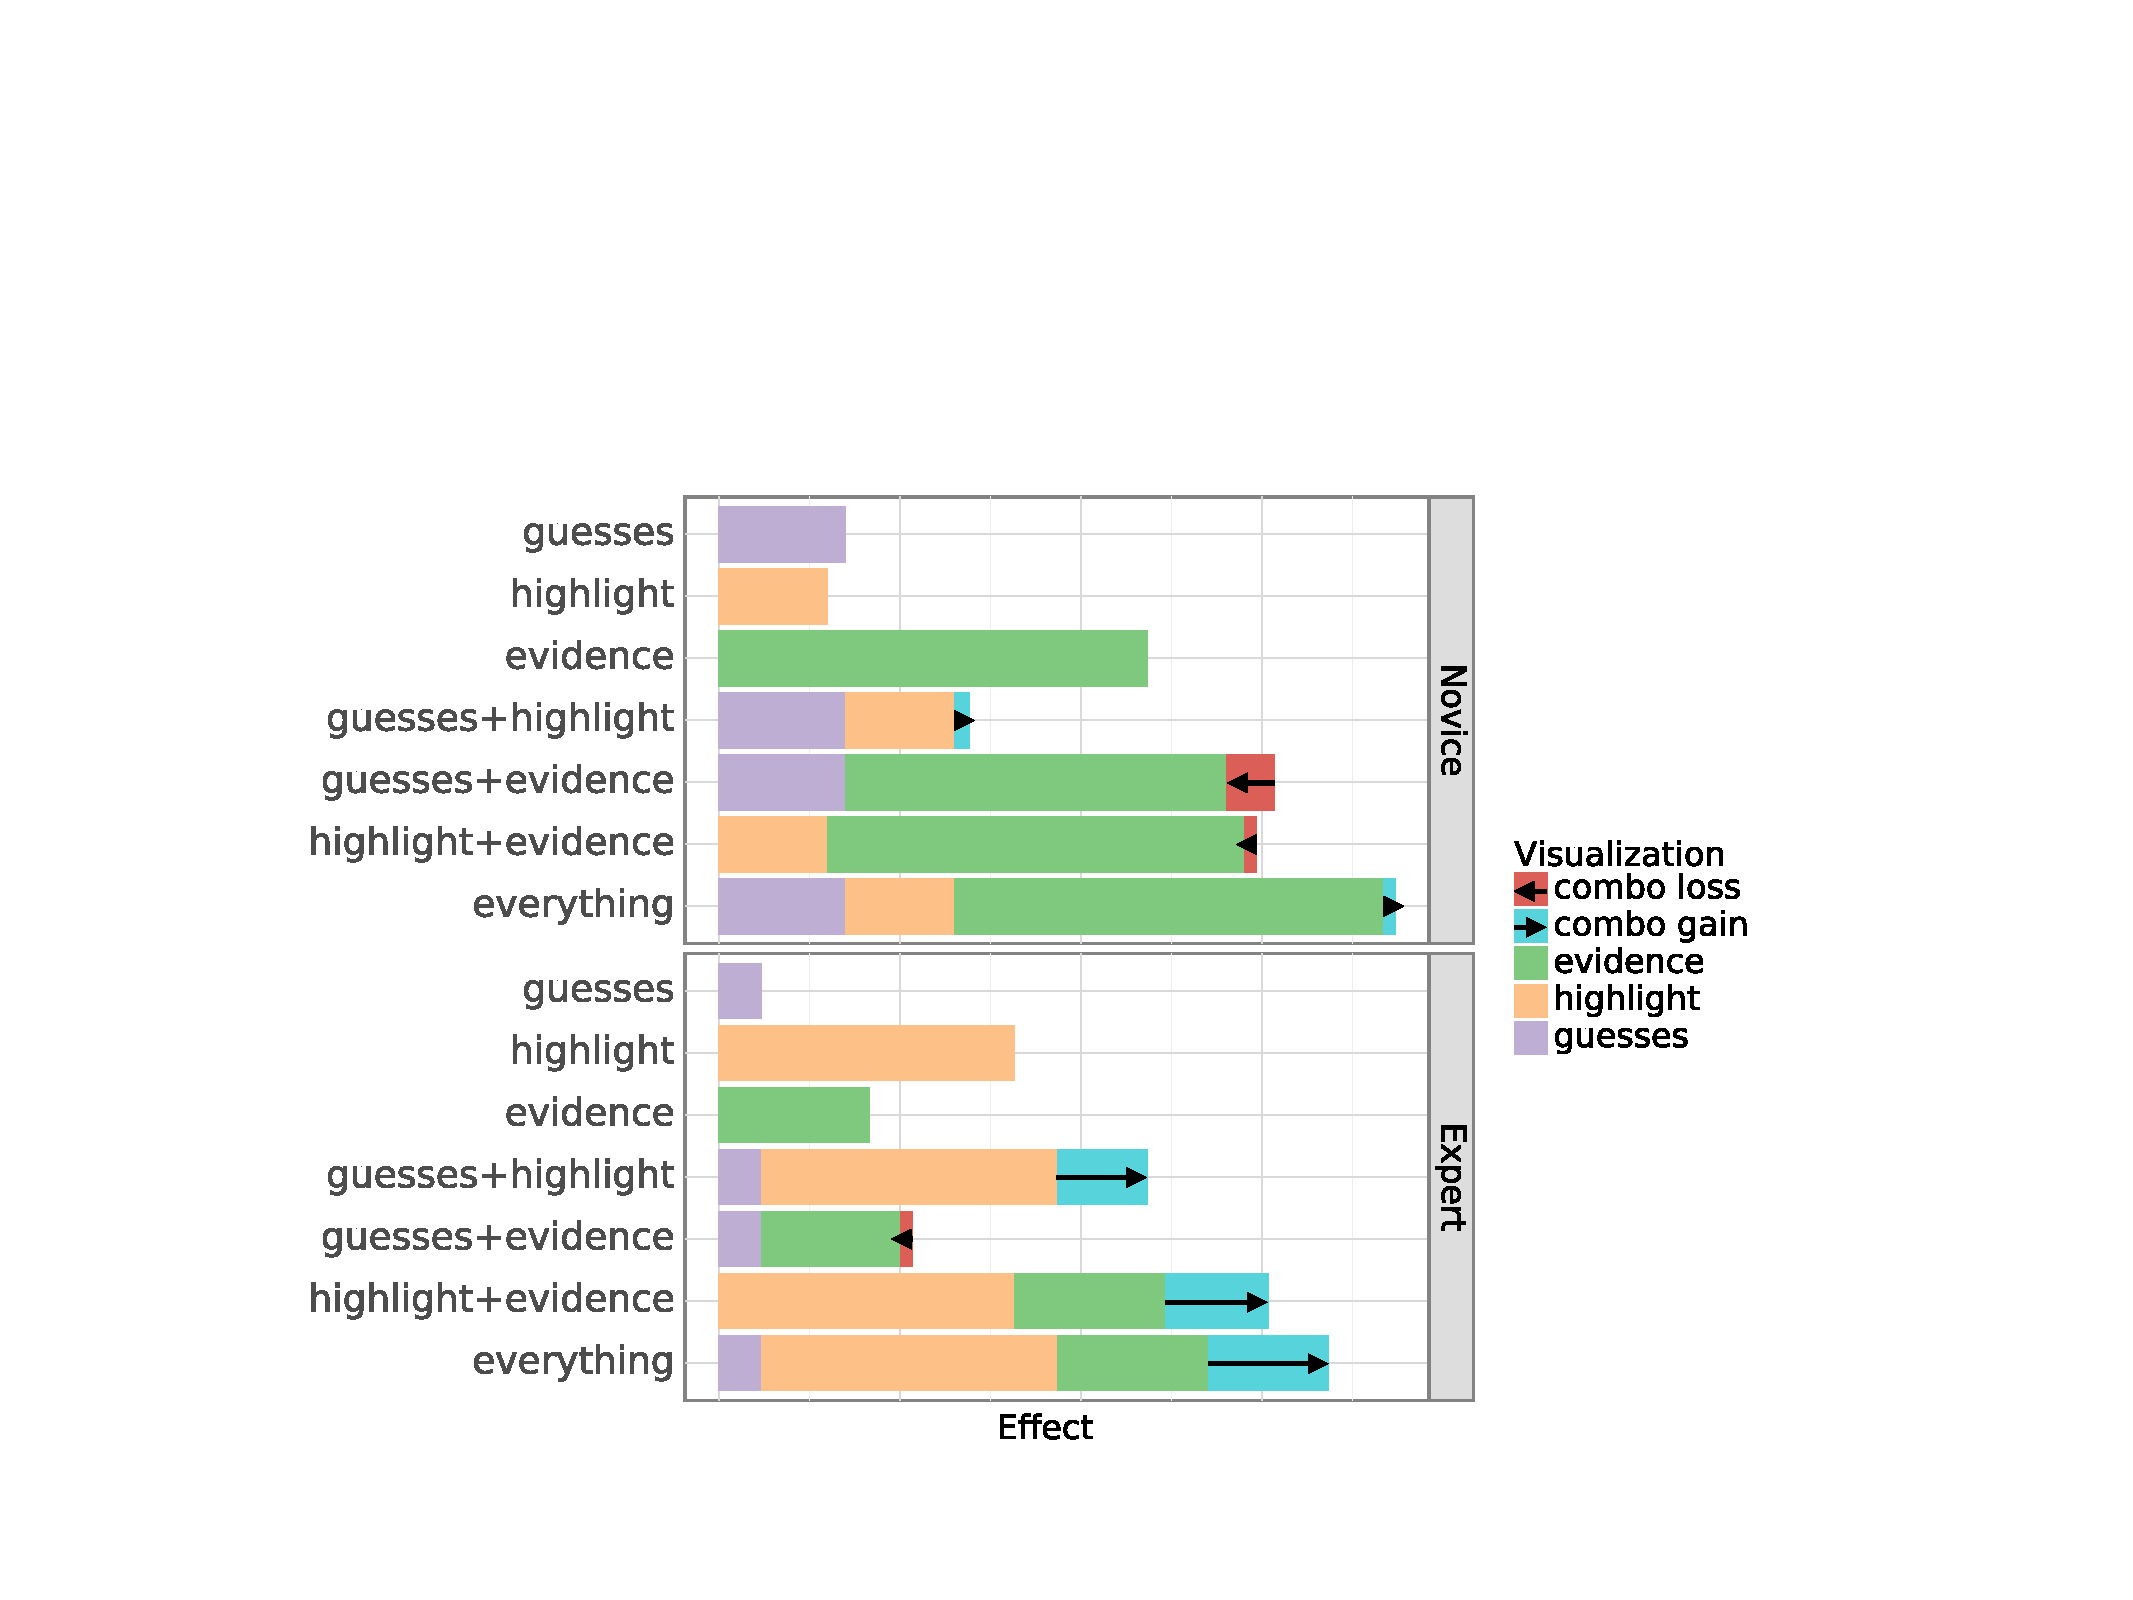
\includegraphics[width=1.0\columnwidth]{coefs_new}
    \caption{\label{fig:coefs} Coefficients of the linear regression
    showing the effects of interpretations, for novices (above) and
    experts (below).
    Higher value means an interpretation improves player accuracy.
    In addition to the individual interpretations, \emph{combo gain}
    and \emph{combo loss} capture the additional effect of combining
    multiple interpretations. \emph{Highlight} and \emph{Evidence}
    are effective for both novices and experts; combining leads to
    more positive effect for experts than novices, potentially because
    experts can process more information in limited time.}
\end{figure}

\begin{figure}[t]
    \centering
    \textbf{Effect of player ability}\par\medskip
    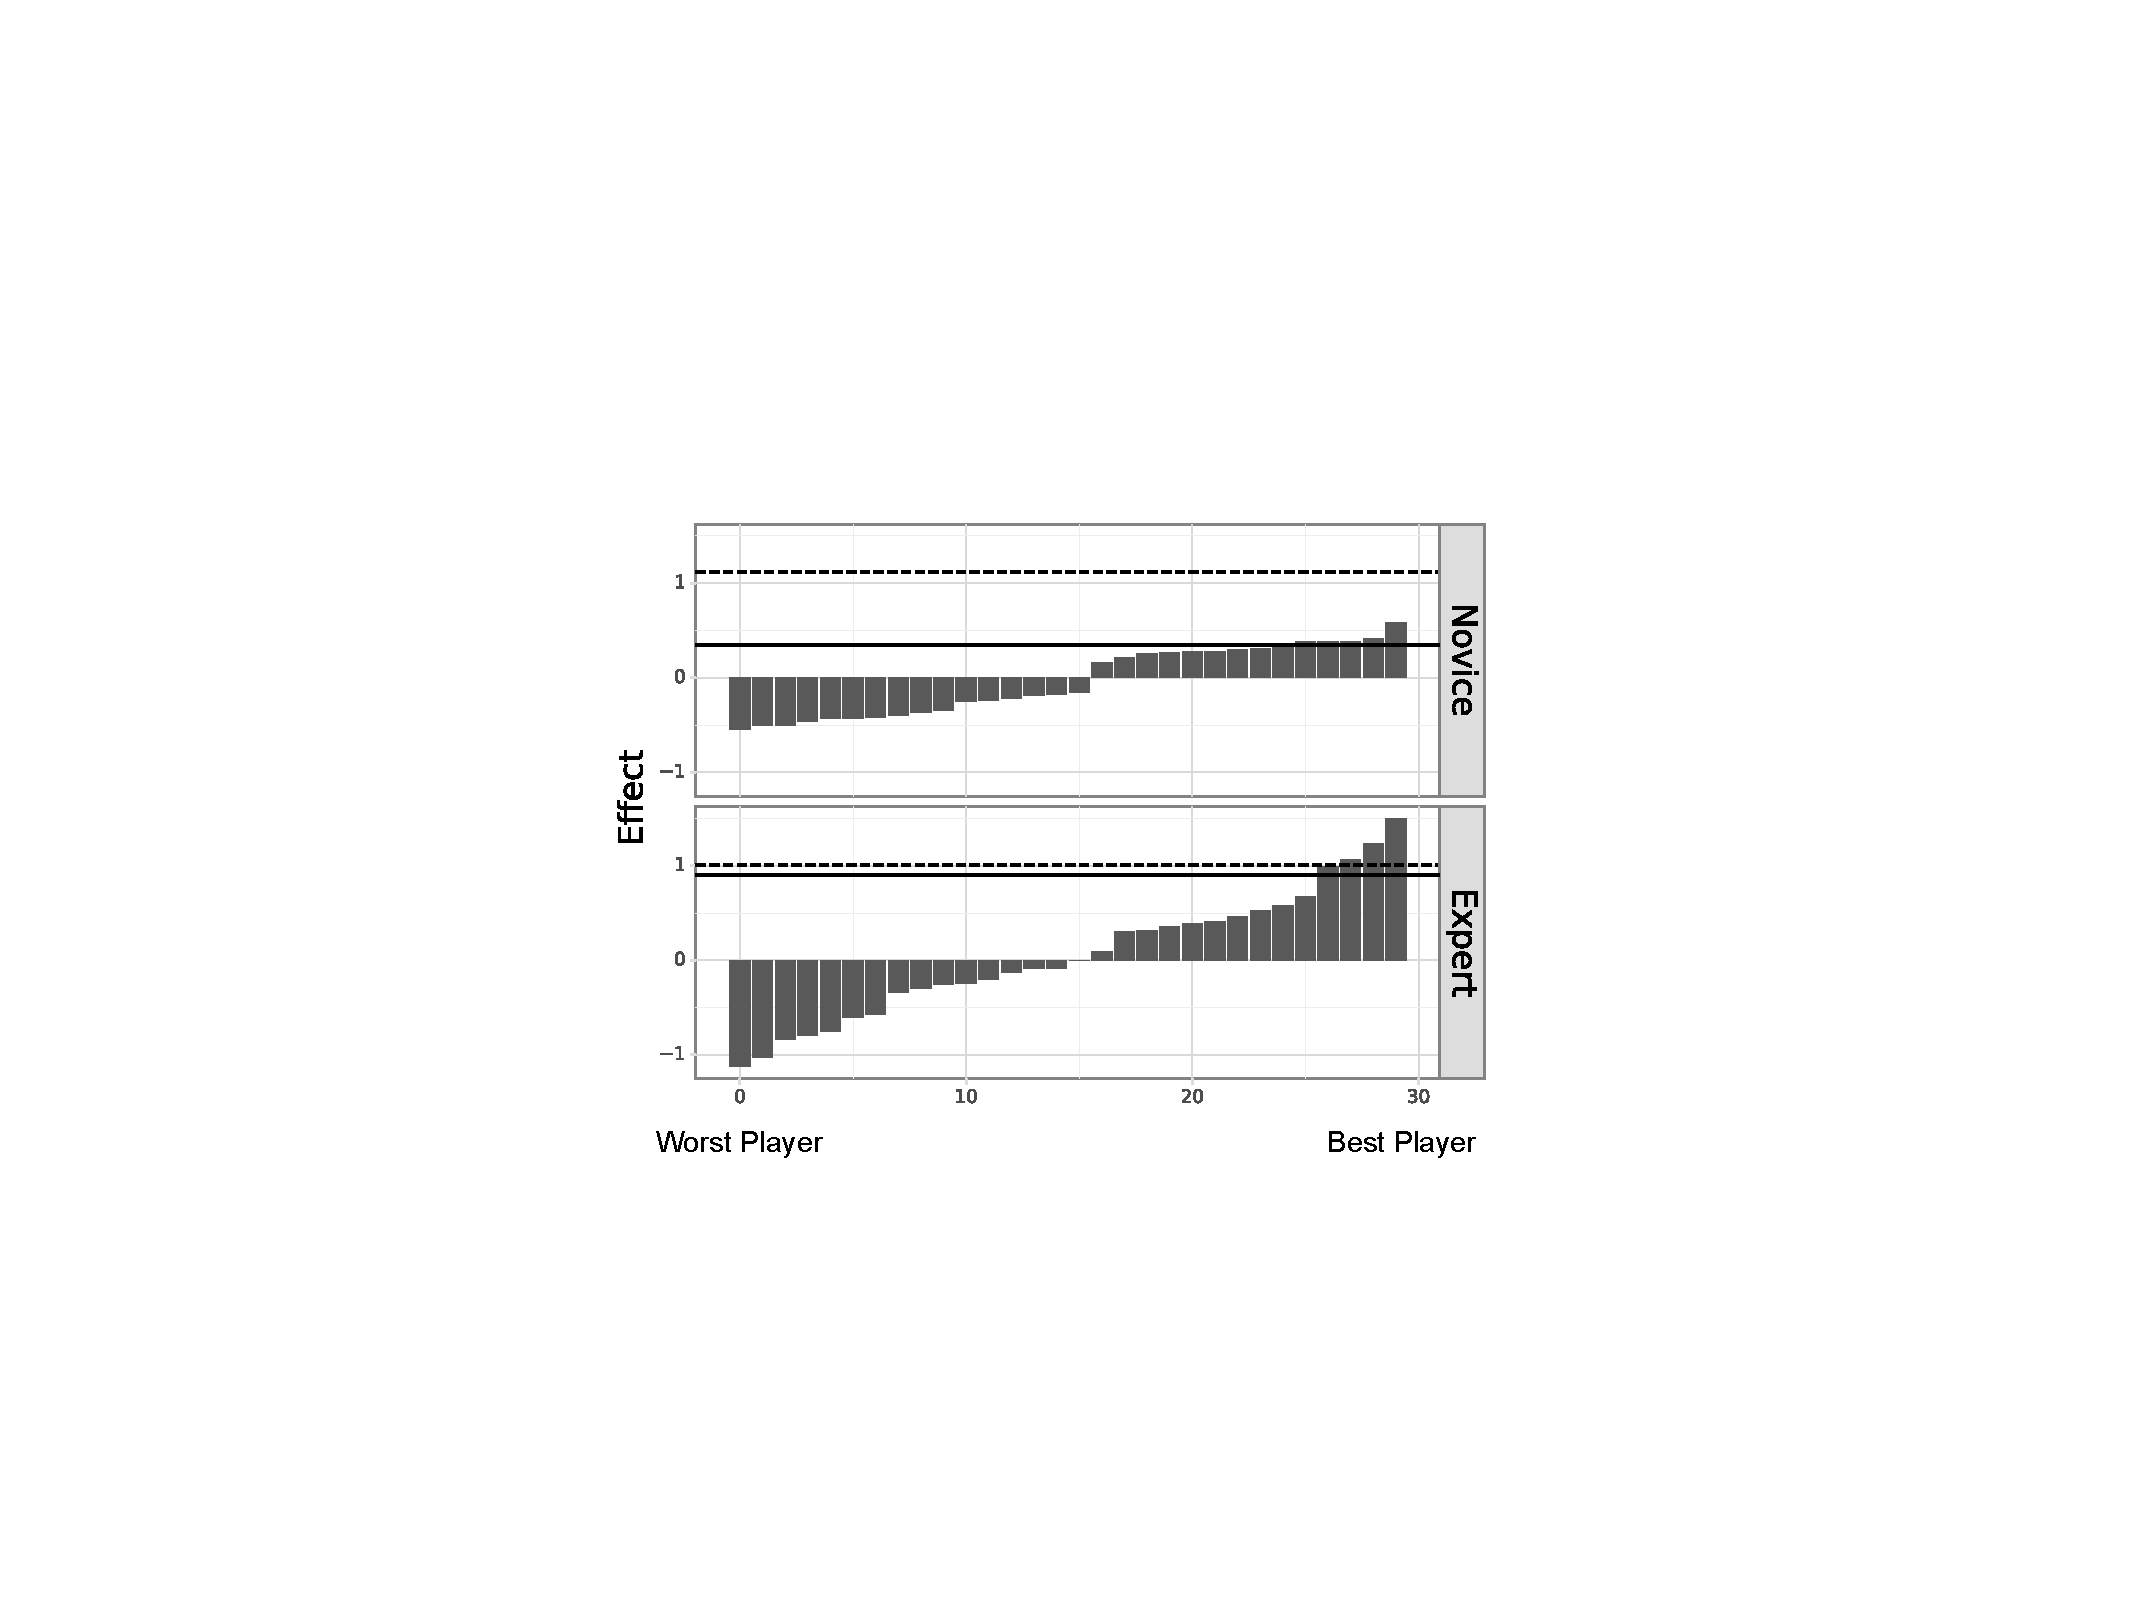
\includegraphics[width=.7\columnwidth]{u_coefs_new}
    \par\medskip
    \textbf{Effect of question difficulty}\par\medskip
    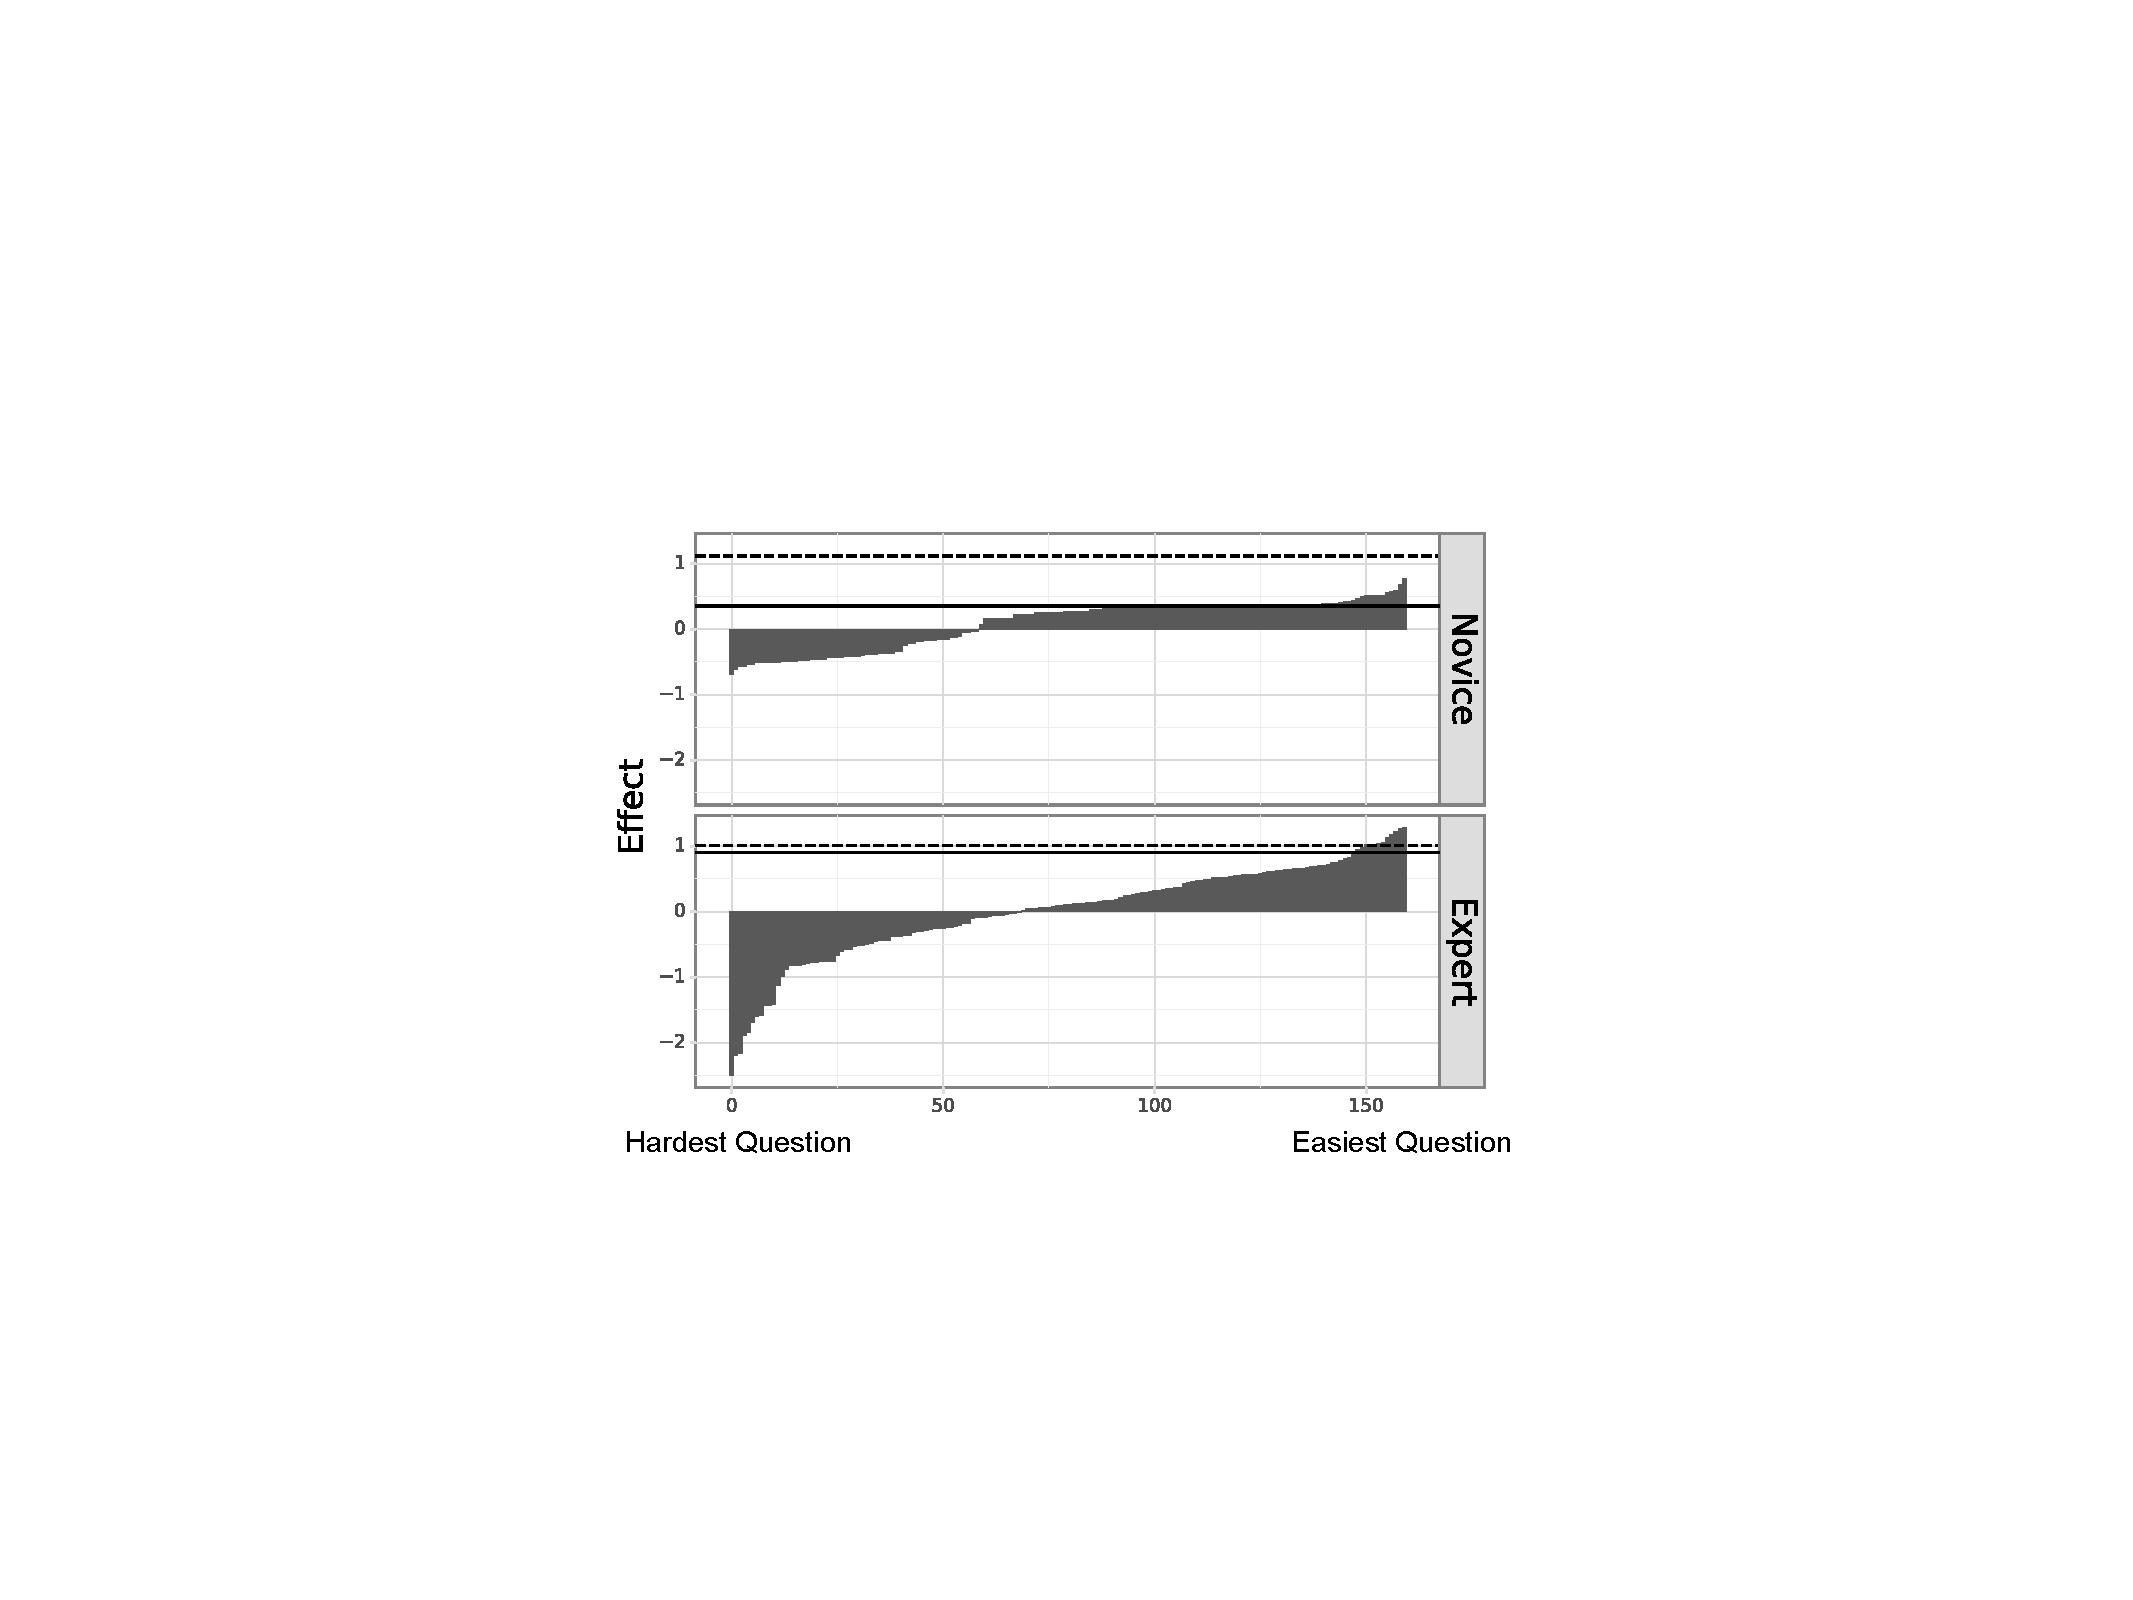
\includegraphics[width=.7\columnwidth]{q_coefs_new}
    \caption{\label{fig:uq_coefs} Effect of player ability (above) and
    question difficulty (below) from the regression analysis. Solid
    horizontal lines show the bias term that captures the baseline
    accuracy without any help from the computer;
    dashed lines show the effect of combining all
    interpretations.  Experts have a higher average accuracy; they are
    also less affected by interpretations.}
\end{figure}

% \begin{figure}[t]
%     \centering
%     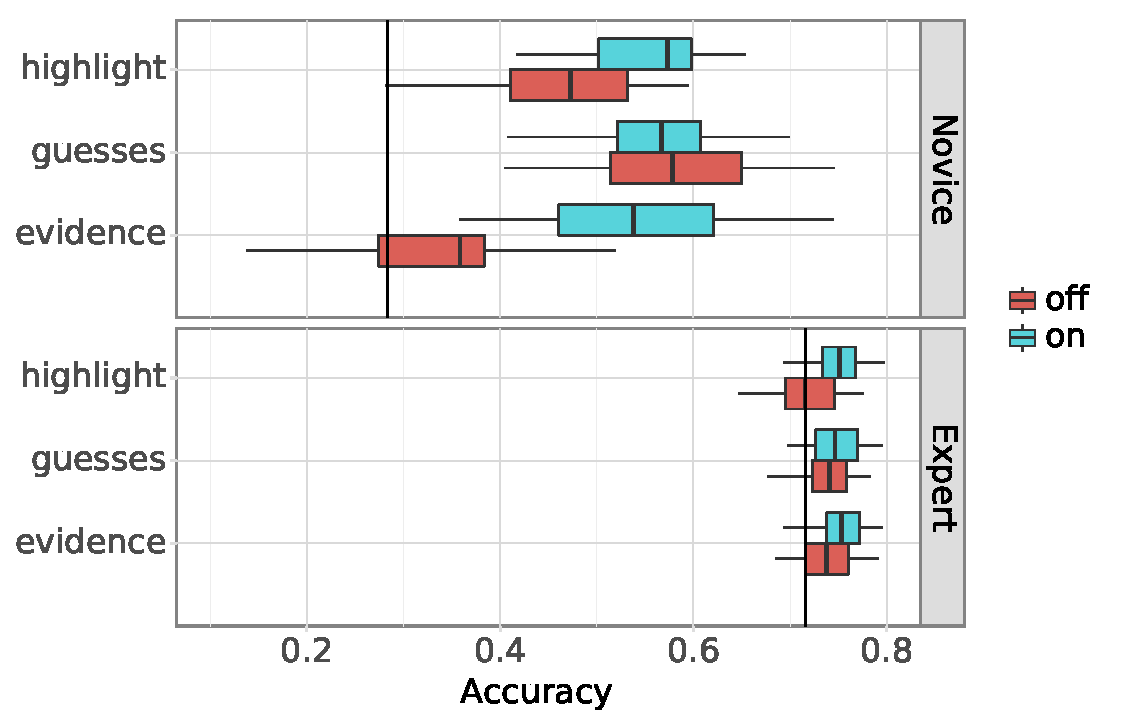
\includegraphics[width=\columnwidth]{tools_acc}
%     \caption{\label{fig:tools_acc} Accuracy of novices (above) and
%     experts (below), with and without each interpretation. One
%     interpretation being \emph{On} means that the interpretation is
%     shown to the players (possibly in combination with others); other
%     interpretations can still be used if one of them is \emph{Off}.
%     Vertical bars show the baseline accuracy without any
%     interpretation.
%     Unsurprisingly, experts show higher performance than novices and
%     are more consistent. Among the interpretations, evidence
%     significantly improves novice performance.}
% \end{figure}

\begin{figure}[t]
    \centering
    \textbf{Distribution of buzzes}\par\medskip
    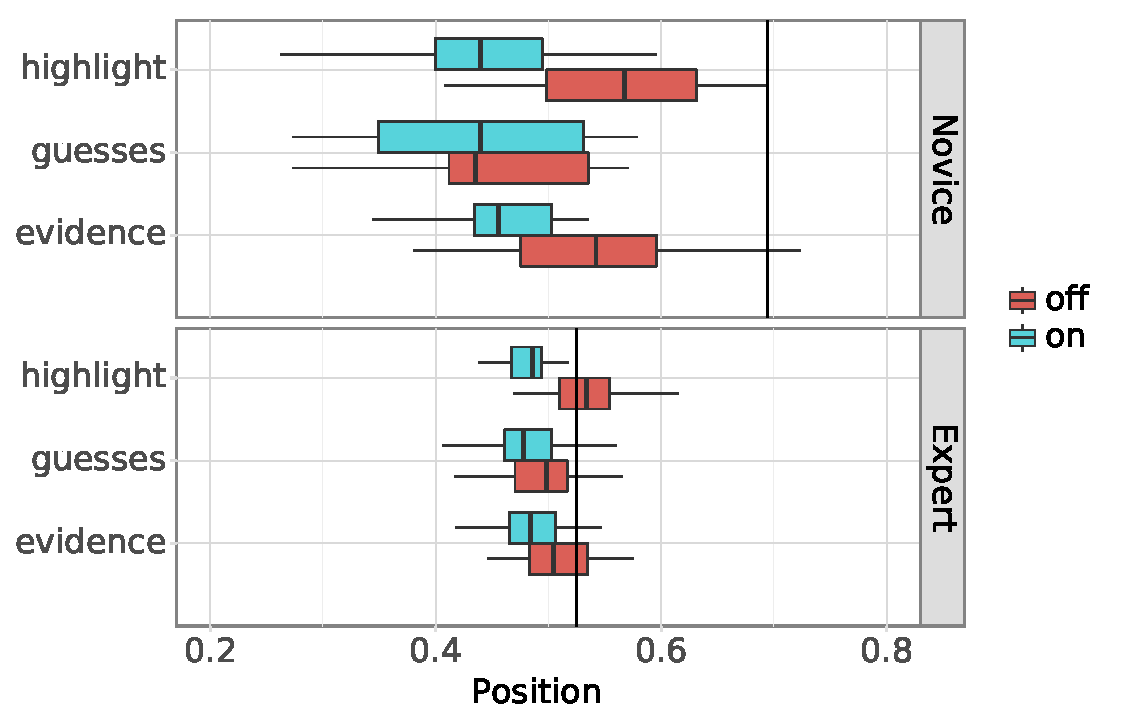
\includegraphics[width=\columnwidth]{tools_buzz}
    \caption{\label{fig:tools_buzz} Average buzzing position (relative
    to question length) of novices (above) and experts (below),
    with and without each interpretation. The goal is to buzz as early
    as possible.
    Vertical bars show the baseline buzzing position without any
    interpretation.
    % Like Figure~\ref{fig:tools_acc},
    Experts are better and more consistent.
    Among the interpretations, \emph{Highlight} is
    most effective in helping both novices and experts answer faster.}
\end{figure}

\begin{figure}[t]
\centering
\textbf{Aggressiveness of novice buzzes}\par\medskip
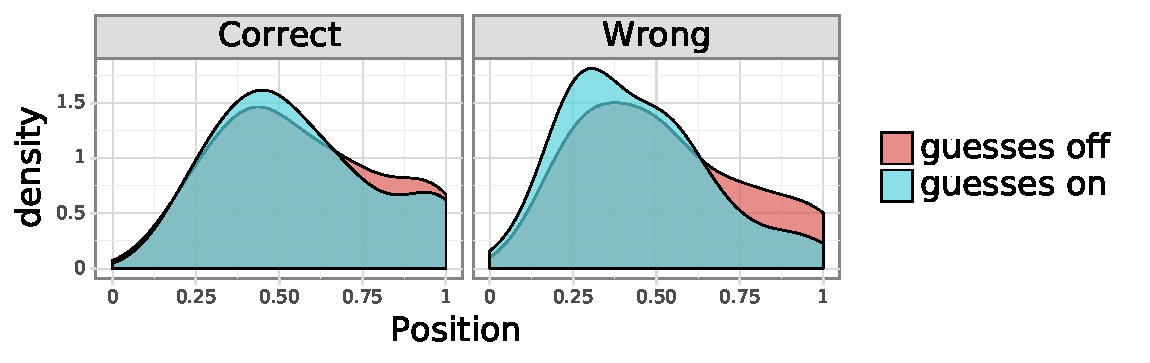
\includegraphics[width=.8\columnwidth]{novice_form_guesses}
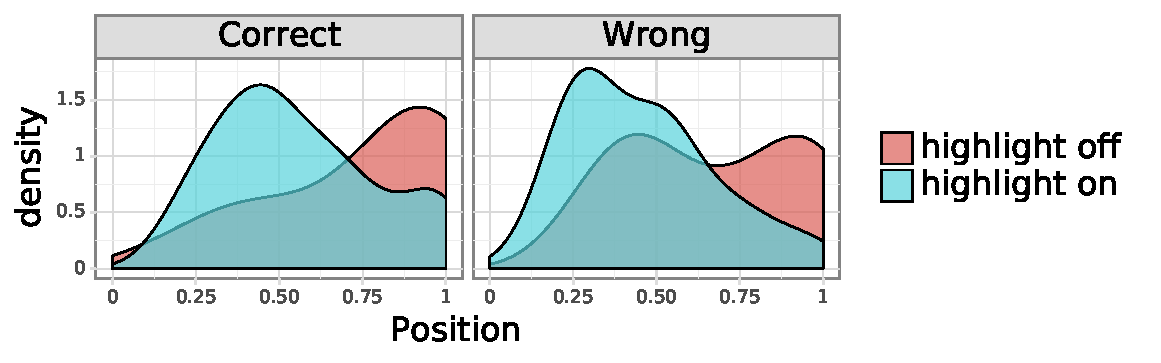
\includegraphics[width=.8\columnwidth]{novice_form_highlight}
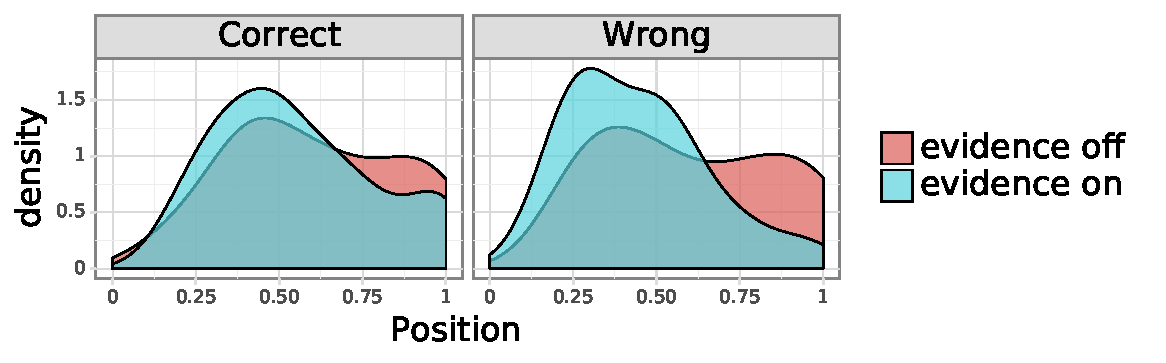
\includegraphics[width=.8\columnwidth]{novice_form_evidence}
\caption{\label{fig:aggressive_novice} The distribution of buzzes of
    novices on correct guesses (left) and wrong guesses (left); colors
    indicate if each interpretation is enabled; positions are
    normalized by question length.  With interpretations, novices are
    significantly more aggressive, but also get more questions correct
    earlier. \emph{Highlight} is the most effective.}
\end{figure}

\begin{figure}[t]
\centering
\textbf{Aggressiveness of expert buzzes}\par\medskip
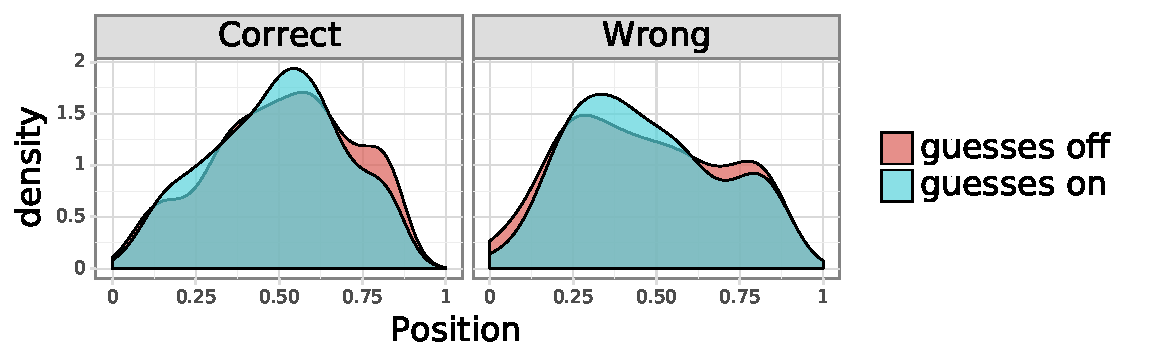
\includegraphics[width=.8\columnwidth]{expert_form_guesses}
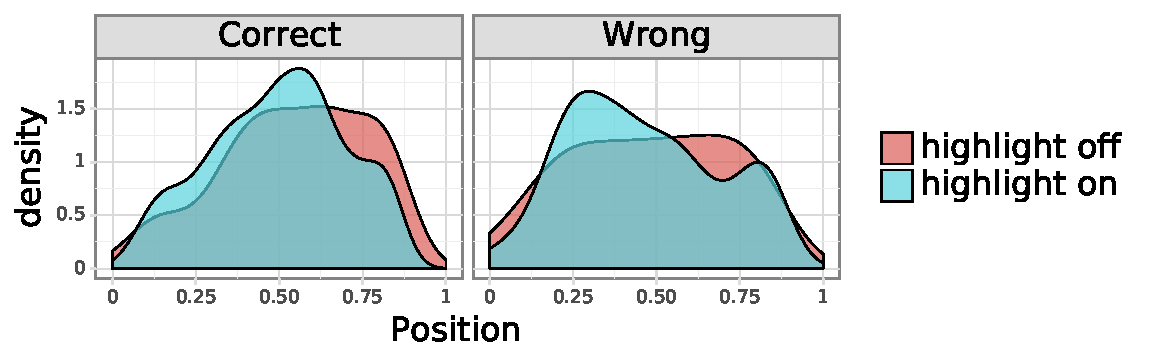
\includegraphics[width=.8\columnwidth]{expert_form_highlight}
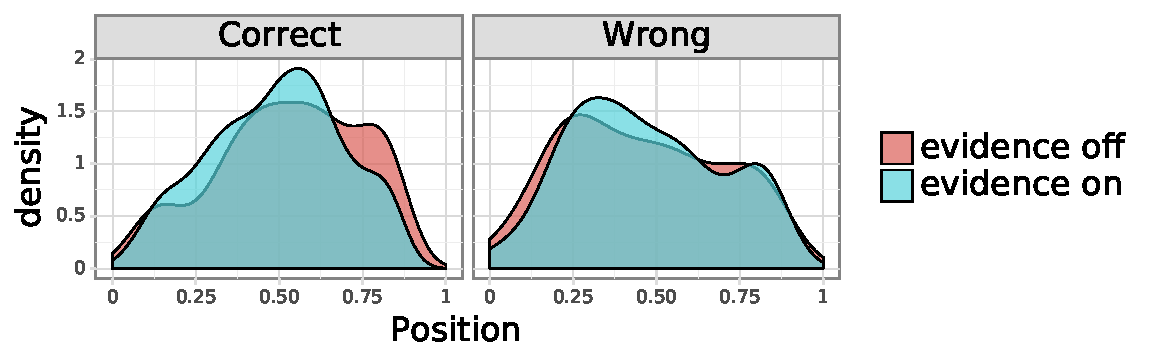
\includegraphics[width=.8\columnwidth]{expert_form_evidence}
    \caption{\label{fig:aggressive_expert} The distribution of buzzes
    of experts on correct guesses (left) and wrong guesses (left);
    colors indicate if each interpretation is enabled; positions are
    normalized by question length.  Experts are not significantly
    more aggressive with interpretations, but they did get more answers
    correct earlier.}
\end{figure}

% 1. overview of what we do in this section
With data collected from game plays, our primary goal is determine if
the interpretations are helpful or not, and how experts and novices
used them differently.
We first do a regression analysis to
quantitatively determine how much each condition affects the
accuracy of the players; then we break down the results to see
how the players behave differently under the conditions, specifically
how aggressive they are; we also look at specific cases where some
interpretation consistently succeeded or failed to convince multiple
players of the model prediction.

% 2. raw data description, using all numbers here for consistency
After filtering players who answer very few questions, we arrive at
30 experts that answer 1983 questions, and 30 novices that answer
600 questions. Turkers usually stopped after answering the required
twenty questions, but many experts kept on playing. Among all players,
seven experts answer all 160 questions.

\subsection{Regression Analysis}

% 3. motivate regression analysis
Whether a player can answer a question correctly is determined by
several factors: the player's innate skill, the difficulty of the
question, the aid of some interpretation, or the competitive level (in
expert setting).  To tease apart these factors we follow
Narayanan~\etal{}~\cite{narayanan2018humans} and apply a regression
analysis.

\begin{table}
\begin{tabular}{l|l}
\multirow{5}{*}{\begin{tabular}[c]{@{}l@{}}Interpretation\\ (8)\end{tabular}} & none, guesses, highlight, evidence,     \\
                                                                              & guesses + highlight,                    \\
                                                                              & guesses + evidence,                     \\
                                                                              & highlight + evidence,                   \\
                                                                              & guesses + highlight + evidence          \\ \hline
\multirow{2}{*}{Player (30)}                                                  & player IDs                              \\
                                                                              & (separate for experts and novices)      \\ \hline
Question (160)                                                                & question IDs                            \\ \hline
\multirow{5}{*}{Others (3)}                                                   & buzzing position                        \\
                                                                              & (relative to question length),          \\
                                                                              & number of active players (expert only), \\
                                                                              & current accuracy of the top             \\
                                                                              & active player (expert only)
\end{tabular}
\caption{\label{table:features} Our four sets of features used in
regression analysis. Numbers in the parentheses indicate the number of
features in that set.}
\end{table}

% 4. features
We describe these factors using the four sets of features listed in
Table~\ref{table:features}.
To capture the player's innate skill and the difficulty of the
question, we include the IDs of both in the feature set.  Each
combination of interpretations has its own features, for example,
\emph{guesses}, \emph{evidence}, and \emph{guesses+evidence} are three
independent features.  For game condition, the first feature is the
relative position in the question when the player buzzed (to
understand how interpretations affect buzzing position as an outcome
instead of feature, we use a separate analysis); for the expert
setting, we also include extra features to capture the
competitiveness: number of active players and the current accuracy of
the top active player.

% 5. the output
The we use a linear model to predict whether the player can answer the
question correctly.  Specifically, for each game record, we extract
the features and feed the vector as input to the linear model, which
then predicts the probability of a positive result; to train the
model, we compare the prediction against the ground truth, and update
the model with gradient descent.  We train this model on the game play
data, for experts and novices separately.

% 6. interpreting regression
The coefficients of the linear model then explains the
importance of the corresponding features: the probability of a
positive result increases with features with positive coefficients, which
means these features help the players. Similarly negative coefficient
means the features hurt the player accuracy.  To understand which
interpretations are most helpful to \qb{} players, we inspect the sign
and magnitude of their corresponding coefficients.

% 7. explain figure
Figure~\ref{fig:coefs} shows the effect of interpretations based on
regression coefficients: a high positive weight means the
interpretation is useful, zero means it is ineffective, and negative
means it is harmful.
It is not guaranteed that the strengths of multiple interpretations
are combined when they are displayed at the same time.
This is due to confounding factors such as information load---the
player might feel distracted when too much information is displayed on
the interface and thus perform worse.
The additional effects of combining
interpretations are ``combo gain'' and ``combo loss''
(Figure~\ref{fig:coefs}).
For example, combining guesses and evidence has a negative effect on
novices; the loss is computed by comparing the ``guesses+evidence''
coefficient with the arithmetic sum of the ``guesses'' and
``evidence'' coefficients.

% 8. findings about experts vs novices
The interpretation that helps novices is not the same as what helps
experts.  For experts, highlight is the most helpful individual
interpretation, while for novices, evidence is the most helpful. For
experts, the combination of highlight and evidence achieves extra
gain, which is reasonable because this combination adds
highlights to the evidence, making the contrast more intuitive.
However, the same combination does not show additional benefit for
novices, potentially due to information overload.

% 9. non-concrete finding
We hypothesize that the main difference between experts and novices is
that experts can use evidence more effectively. 
Question highlighting requires less
multitasking than evidence: players have to look away from the
question they need to answer to take in the evidence.  \qb{} players
likely know when they can glance down to related training data and can
also determine whether the training data are helpful.

% 10. non-interpretation factors
To understand how much variance players display in their skill and
questions in their difficulty, we show their corresponding
coefficients (Figure~\ref{fig:uq_coefs}). The solid horizontal line
shows the baseline accuracy of that player group without any
interpretation (the bias term---or the intercept---of the linear
model). Experts show a higher baseline accuracy, which is not
surprising since they are experts; they also show a larger variance
in accuracy within the group, potentially due to the competitive
environment; they are also more sensitive to the difference in
question difficulty.
To compare these factors against the interpretations, we
show with the dashed horizontal line the combination of all three
interpretations. Experts are less sensitive to the interpretations,
potentially due to a higher confidence in their own guesses.

\subsection{How Interpretations Change Player Behavior}

% 11. motivate the analysis of buzzing behavior
The regression analysis provides a quantitative comparison between all
interpretations in how they affect the player accuracy. However,
accuracy alone does not tell the full story of how they play the
game. This section describes how each
interpretation affects the behavior of the players and how the effect
differs for novices and experts.  Ideal players should be both
aggressive and accurate: seeing very few words and answering
correctly. Interpretations should help them reach this goal.

% 12. buzzing position with and without
Figure~\ref{fig:tools_buzz} show the
average buzzing position of each player group with and without each
interpretation.
% The effect of each
% interpretation on the accuracy of experts and novices concurs
% (Figure~\ref{fig:coefs}).
Novices buzz much later than experts when no interpretation is enabled
(comparing the solid vertical bars), but buzz at about the same point
as experts when interpretations are enabled, despite a lower accuracy
(Figure~\ref{fig:uq_coefs}). This suggests that the novices are too
trusting in the computer teammate, and end up playing too aggressively
for their skill level.

% 13. buzzing position density
We see a similar trend when we plot the density 
of buzzing positions (experts in Figure~\ref{fig:aggressive_expert}
and novices in Figure~\ref{fig:aggressive_novice}). In all settings,
the density shifts earlier: players are more aggressive with
interpretations, especially for novices, which is consistent with
Figure~\ref{fig:tools_buzz}. The interpretations allow players to
answer correctly earlier. Especially for novices with
highlights, the distribution of correct buzzing positions shifts
significantly earlier in the questions.

% 14. novices are too trusting
Although novices are helped by visualizations, these visualizations
are not enough to help them discern useful help from misleading help.
Novices are too aggressive at the start of the question with
visualizations: they trust the predictions of the system too much.
While experts mentally tune out bad suggestions, novices
are less discerning.  Visualizations thus 
must also convey whether they should be trusted, not just what answer
they are suggesting.

\subsection{Successes and Failures of Interpretations}

We now examine specific cases where interpretations help or hurt
players.

\begin{figure}[t]
\centering
\tikz\node[fill=white!70!colorsquad,inner sep=1pt,rounded corners=0.3cm]{
\begin{tabular}{p{0.46\textwidth}}
\emph{Question}:\\
(This essay) was composed after its author \textbf{refused} to
pay a \textbf{poll tax} to support the \textbf{Mexican-American}
\textbf{war}, and its ideology inspired Martin Luther King, Jr.\
and Mohandas Gandhi. \\

\emph{Evidence}:\\
him to pay six years of delinquent \textbf{poll tax}. Thoreau
\textbf{refused} because of his opposition to the
\textbf{Mexican-American War} and slavery, and he spent a night
in jail because of this refusal.
\end{tabular}
}; % end of tikz node
\caption{\label{fig:success} Interpretations that help players answer
a question on \underline{Civil Disobedience} correctly.  With the
shown part of the question, three experts answer correctly with the
evidence; no expert answer correctly without.}
\end{figure}

Figure~\ref{fig:success} shows an example where interpretations enable
players to answer correctly. A total of twelve expert players
answered the question, and eight answered correctly. The
earliest an expert can answer correctly without the evidence was at 72\%
of the question, while the three experts with the evidence all
answer correctly before 50\%. With the evidence and highlight,
players can infer from the keywords that the author is
Thoreau and that the guess is likely correct.  The computer shows
a salient training example and is effective in convincing the players
that the retrieved evidence is correct.

\begin{figure}[t]
\centering
\tikz\node[fill=white!70!colorsnli,inner sep=1pt,rounded corners=0.3cm]{
\begin{tabular}{p{0.46\textwidth}}
\emph{Question}:\\
A \textbf{book} by this man was first published with a
\textbf{preface} by Andreas Osiander titled \textbf{Ad Lectorem}.
\\
\emph{Evidence}:\\
the \textbf{Ad Lectorem} \textbf{preface} to Copernicus's
\textbf{book} was not actually by him.
\end{tabular}
}; % end of tikz node
\caption{\label{fig:fail_to_convince} Interpretations that fail to
    convince players.  Three expert players, when presented with the
    interpretation (some question text and evidence omitted), rejected the
    computer's correct guess (\underline{Copernicus}) and answered
    differently.}
\end{figure}

Figure~\ref{fig:fail_to_convince} shows a failure to convince,
where the combination of highlight and evidence fails to convince the
player of the computer's \emph{correct} guess: three expert players
rejected the computer's prediction and provided different answers,
relatively early in the question (before 50\%). The information
provided by the evidence is that Copernicus has a book with a
preface named Ad Lectorem, this piece of evidence strongly supports the
computer's guess \underline{Copernicus}.  However, it is expressed
differently than the question, with an unrelated but confusing ``not''
in the middle of the sentence.

% \jbgcomment{There needs to be more of an in-depth analysis.  Find:
%
% \begin{enumerate}
%   \item A player who is so good that no interface element helps
%   \item A super easy question
%   \item A very difficult question
%   \item Questions that suddenly become answerable with additional evidence, show the evidence that made it answerable
% (many of these can be found by looking at outliers)
% \end{enumerate}
%
% }

% \begin{table}[t]
% \centering
% \begin{tabular}{lll|ll}
%           & \multicolumn{2}{c|}{Accuracy}                           & \multicolumn{2}{c}{Position}                           \\
%           & \multicolumn{1}{c}{With} & \multicolumn{1}{c|}{Without} & \multicolumn{1}{c}{With} & \multicolumn{1}{c}{Without} \\ \cline{2-5}
% Guesses   & 0.7481                   & 0.7434                       & 0.5817                   & 0.5981                      \\
% Highlight & 0.7506                   & 0.7182                       & 0.5839                   & 0.6306                      \\
% Evidence  & 0.7487                   & 0.7380                       & 0.5813                   & 0.6134
% \end{tabular}
% \caption{Average accuracy and buzzing position (divided question length),
%     with and without each tool. Lower value in buzzing position indicates more
%     aggressive playing.}
% \label{table:form_acc_pos}
% \end{table}
